\chapter{Supervised Machine Learning}
\label{chapter:SupervisedLearning}

In Chapter \ref{chapter:Motivation}, we briefly reviewed the areas that
constitute the field of \ac{ml} and motivated an introductory example to
\acl{rl}. We highlighted the differences between \ac{sml} and \ac{rl} by
contrasting the way each work. \Ac{sml} receives a wealth of examples from which
it must extract patterns, while \ac{rl} receives no input data and so has to
learn by interacting with its environment. Statistically speaking, \ac{sml} is
often tasked with classifying or predicting a response. In this thesis, we focus
only on the classification task.

\section{Classification}

\Ac{sml} algorithms tasked with classifying receive large amounts of
labeled data. Through the process called ``fitting'' or ``learning'', the
algorithm will (hopefully) label correctly new observations never seen before.
The classification task seeks to find a systematic way of predicting a
phenomenon given a set of measurements.

\subsection{A formal description} \label{sss:formalizing-trees}

Putting some concepts to work, picture a scenario where we have access to
several measurements (e.g., age, weight, blood pressure, etc.) for a group of
patients. Some patients in the study group suffered a stroke; the rest did not.
Our task is to find a systematic way of predicting whether or not a new patient,
not seen before, will suffer from a stroke by measuring the same variables
measured for the initial group.

Fundamentally, \iac{sml} algorithm must receive a \textit{training set}, a set
of pre-labeled data from a knowledgeable source, in contrast with \ac{rl}, where
labeling is often not even possible or practical. This source of truth, the
training set, is a set of observations $(\vec{x}_1, y_1), \dots, (\vec{x}_n,
y_n)$. The vectors $\vec{x}_i = [x_{1, i}, x_{2, i}, \dots, x_{p, i}]^{\top} \in
\R^{p}$ can be thought of as a list of measurements of every variable of
interest for the $i$-th patient. In the case of the example trying to predict
strokes, $x_{1, i}$ would correspond to age and $x_{2, i}$ to weight for the
$i$-th patient. The training set also contains $y_1, \dots, y_n$,
one-dimensional values we call responses or labels in the specific case of
classification. Using the standard parlance, the input variables are known as
\textit{features}, input vectors as \textit{instances} or \textit{samples} and
the output variable as \textit{target}.

For the purposes of this thesis, we consider that the target variable is always
categoric, not numeric nor continuous. Nevertheless, continuous target variables
are allowed, but the learning task is called regression, which is outside this
thesis's scope. To make the description of the algorithms easier, we concentrate
on the classification case where all features are continuous, not categoric.

In a typical \ac{ml} workflow, the algorithm used to make predictions is trained
on the set we just described. Its performance is tested on a different set of
similar data that the algorithm had no access to during its training period.
From now on, we denote the training set as $\L$. For convenience we group the
feature vectors into a \textit{feature matrix} $X \in \R^{p \times n}$, where
the $i$-th column is $\vec{x}_i$. Similarly, we group the target variables into
the vector $\vec{y} \in \R^{n}$.

Our classification task can be framed as finding a function $f_{\L}$ we will
call model whose output or predictions $f_{\L} (\vec{x}) = \widehat{y}$ are ``as
good as possible''. We subscript the function $f$ with $\L$ to highlight the
fact that the behaviour of the function is highly dependent on what training
data it received. We proceed to define what makes a model ``good'' at making
predictions.

\subsection{Evaluation}

As it has become a recurring theme in this thesis, determining what makes a
prediction suitable and finding the best possible model $f_\L$ is a process of
optimization. 

We will be working under the assumption that the training set is a subset of the
universe of patients for who we can measure the feautures of interest. Under
this assumption we theorize that a model that misclassifies as little as
possible the patients in the training set will also minimize misclassifications
for other patients from the rest of the universe. In reality, this is not
precisely the case, as often making the number of classification mistakes as
small as possible in the training set results in a model that ``memorized'' the
set and has no ability whatsoever to generalize patterns. It only reproduces
known-to-be-good answers. But the idea is not entirely misguided, it provides a
good starting point.

The process we referred to as ``fitting'' a model consists of finding a model
which minimizes its expected prediction error, also called generalization error.
We hope that by minimizing this error we can extract as much information from
the training set without hard-coding the labels for future observations.

\begin{dfn}{Prediction or Generalization Error}{generalization-error}
    The expected \emph{prediction} or \emph{generalization} error of a model
    $f_\L$ is the probability of misclassification of the model
    \[
        \Err (f_\L) = \mathbb{E} \left[ \1 (y_i \neq \widehat{y}_i)  \right].
    \]
    Where $\widehat{y}_i \coloneqq f_\L (\vec{x}_i)$ is the model's prediction
    for the, previously unseen, observation $\vec{x}_i$, and the indicator
    function $\1$ equals one whenever the condition inside it holds, and zero
    otherwise.
\end{dfn}

Minimizing this Generalization Error will allow us to classify the newest
observations committing the lowest possible number of errors overall.
Including observations never seen before, not only the ones we have access to in
the training set. Since the distributions for observations $(\vec{x}_j, y_j)$
are generally not known, we must estimate the generalization error. Several
techniques to solve this problem exist but are numerous and outside of scope.
From now on, we denote by $\widehat{\Err}$ an estimator of the generalization
error.

The term ``fitting'' when discussing finding a suitable model is a consequence
of how such a model is found. Since the generalization error is not directly
measurable and thus not directly minimizable, we have to use a reasonable
approximation. We assume that a family of candidate models, $\mathcal{H}$ known
as hypotheses, exists. Our optimization target then becomes to find the best
model among the space of hypotheses. To be more specific, let $\vec{\theta}$ be
the vector of hyper-parameters controlling the behavior of a specific model in
$\mathcal{H}$.  Then, our optimization task is to find $\theta^{*}$,
\[
    \theta^{*} \coloneqq \argmin_{\theta} \; \widehat{\Err}\left(f_\L (\vec{x}; \theta) \right) \quad \text{ for all } \vec{x} \in \mathcal{X}.
\]
where the vectors of features come from the input space $\mathcal{X}$ defined
clearly in the next section.

Many classification models are available, each leveraging different properties
and resulting in different strengths and weaknesses. The optimization problem
involved in fitting each one may be different from the rest. For this thesis, we
focus on one specific model called classification trees. We introduce them here
and show in part \ref{part:II} how fitting them gives way to an optimization
process analogous to a Reinforcement Learning problem and frame it as such so we
can leverage the power of \ac{rl} to fit classification trees.

\section{Classification Trees}

Classification trees and, more generally, \acf{cart} are \ac{ml} models like the
ones described in the previous section.  They have gained massive popularity in
the recent and ongoing boom in machine learning for their numerous qualities.
For instance, they can model arbitrarily complex relationships in data, handle
both numeric and categorical data, and are easily interpretable as they result
in simple decision rules. Most importantly, they are the building block of
state-of-the-art algorithms for \ac{ml}, such as XGBoost \cite{XGBoost}.

Sadly, their fitting process leads to a rather complicated problem that cannot
be solved exactly in a reasonable time. The fitting process shares many
similarities with the \ac{rl} problem, which is described in detail in Chapter
\ref{chapter:ReinforcementLearning}. This similarity is the foundational idea of
this thesis, and we hope to show in part \ref{part:II} how an alternative
methodology to fitting trees can be developed by leveraging the techniques used
in \ac{rl}. With that goal in mind, it is time to lay the foundations behind how
trees are structured.

\subsection{Tree models}

Let $\Omega = \left\{ (\vec{x}_i, y_i) \right\}$ be the space of all possible
feature-target pairs. When each feature $y$ is part of a set of categories
$\mathcal{C} \coloneqq \left\{ c_1, c_2, \dots, c_j \right\}$, another way to
look at the classification task is to define a partition over $\Omega$ taking
advantage of the natural distinction our set of categories provides. That
partition can be described as:
\[
    \Omega = \bigcup_{i=1}^{j} \Omega_{c_i},
\]
where each $\Omega_{c_i}$ is defined as $\left\{ (\vec{x}_k, y_k) \mid y_k = c_i
\right\}$.

Similarly, a model $f_\L$ defines a partition. This partition however is made
over the input space $\mathcal{X} = \left\{ \vec{x}_i \mid (\vec{x}_i, y_i) \in
\Omega \right\}$. This partition can be described as the preimages of $f_\L$ as
such
\[
    \mathcal{X} = \bigcup_{i=1}^{j} f_{\L}^{-1}(\{ y \mid (\vec{x}, y) \in \Omega_{c_i} \}) = \bigcup_{i=1}^{j} f_{\L}^{-1}(c_i).
\]
The classification task then can be thought of as fitting the model $f_\L$ that
gives the partition of $\mathcal{X}$ that most closely approximates the
partition on $\Omega$ as a result of its preimages.

We are trying to represent $f_\L$ as a tree (in the same way Computer Science
thinks about trees) where any node $t$ represents a \underline{subset}
$\mathcal{X}_t \subseteq \mathcal{X}$ of the input space such that the node
designated as root (denoted $t_0$) corresponds to the entirety of $\mathcal{X}$.
Recall that in this thesis we focus on the case where all features are numeric,
which allows us to conceptualize $\mathcal{X}$ as a subset of $\R^{p}$ where $p$
is the number of features.

Internal nodes $t$ are originated via a \textit{split} $s_t$ taken from a set of
questions $\mathcal{Q}$.  The set of questions $\mathcal{Q}$ is exactly what it
sounds like. The question defining split $s_t$ might be, for example, is $x_{m,
1} < 65$? Or, is the person recorded as observation $m$ younger than 65? The
space $\mathcal{X}_t$ represented by node $t$ is made up of disjoint subsets
corresponding to each of $t$'s children nodes; two in the case of binary trees. 

Terminal nodes (or leaves) are labeled with a best guess value $\widehat{y}_t
\in \mathcal{C}$. In the case of classification, this prediction value
$\widehat{y}_t$ is usually set as the class $c_k$ shared by the majority of the
observations at that leaf. Since our aim is to minimize generalization error, we
would like nodes to be as ``purely'' one class as possible.

The prediction process is carried out by navigating the tree,
providing answers to the questions defining each node until a leaf is reached.
The label for that leaf will be the tree's prediction. In algorithm
\ref{alg:tree-predict}, we show a formal description of the process of using an
already fitted tree $f_\L$ to predict the label of a new observation. 

\begin{algorithm}
    \SetKwFunction{Predict}{predict}
    \KwIn{The tree $f_\L$}
    \KwIn{The feature vector $\vec{x}$}
    \KwOut{The predicted class $\widehat{y}$ for $\vec{x}$}
    \Function{\Predict{$f_\L, \vec{x}$}}{
        $t \gets t_0$ \;
        \While{$t$ is not a terminal node}{
            $q \gets$ the question in $\mathcal{Q}$ that separates the node $t$. \;
            $t \gets$ the child node $t'$ that corresponds to evaluating $\vec{x}$ at question $q$  \;
        }
        \Return{$\widehat{y}_t$ the value at node $t$} \;
    }
    \caption[Tree prediction algorithm]{Predict output value $\widehat{y}$ with
        tree $f_\L$ \cite[Ch.~3.2]{louppe2014}.}
    \label{alg:tree-predict}
\end{algorithm}

\subsection{Fitting Decision Trees}

\citeauthor{hyafil1976} proved that fitting a decision tree that minimizes the
generalization error is an NP-complete problem \cite{hyafil1976}. That means no
polynomial time algorithm to solve it exists. As with other NP-complete
problems, the solution methods must rely on heuristics. One of the most widely
used algorithms for tree fitting is the \acl{cart} algorithm developed by
\citeauthor{breiman2017} \cite{breiman2017}. Breiman's algorithm is implemented
in scikit-learn\footnote{The industry-standard python library for machine
learning \cite{louppe2014}.}, available to R users via the tidymodels extension
and part of MLJ.jl\footnote{The most widely used machine learning library for
Julia users.}. This chapter explores the \ac{cart} algorithm as a way to fit
decision trees, and part \ref{part:III} of this proposes a new algorithm based
on \ac{cart}.

The \ac{cart} algorithm is based on greedily finding splits based on node
purity, the amount of misclassified observations in a given node. The
\textit{purer} the node, the lower the impurity score, and thus the better the
prediction. We denote by $\L_t$ the subset of the training set $\L$ that
corresponds to a node $t$, defined as:
\[
    \L_t \coloneqq \left\{ (\vec{x}, y) \mid \vec{x} \in \mathcal{X}_t \right\}.
\]

\begin{remark}{Greedy}
    When using the term greedy, we refer to a heuristic used in optimization
    algorithms. The heuristic consists of evaluating the immediately available
    actions without looking ahead to analyze if some action ignores the path
    that will actually lead to the best results down the line. Greedy algorithms
    are often used since looking ahead can be very computationally taxing.
\end{remark}

Many impurity functions can be used to determine the goodness of a split, each
with their benefits and drawbacks. We only discuss the impurity decrease at the
moment, since it is not necessary to have a specific impurity function to
describe the fitting algorithm nor do we have enough space to cover the
available options and their properties.

\begin{dfn}{Impurity decrease}{impurity-decrease}
    The \emph{impurity decrease} $\Delta i$, under an impurity function $i: t
    \subset \R^{p} \to [0, 1]$, of a binary split $s$ of node $t$ into a left
    child $t_L$ and a right child $t_R$, is defined as: 
    \[
        \Delta i(s, t) \coloneqq i(t) - \frac{N_{t_L}}{|\L_t|} \, i(t_L) - \frac{N_{t_R}}{|\L_t|} \, i(t_R),
    \]
    where $N_{t_L}$ and $N_{t_R}$ are the number of observations contained by
    nodes $t_L$ and $t_R$, respectively. The impurity decrease is defined as a
    function of both $t$ and $s$ since the split $s \in \mathcal{Q}$ is what
    defines the children of $t$: $t_R$ and $t_L$.
\end{dfn}

It is straightforward to see the similarity of the impurity decrease definition
with how an expected value is estimated since $N_{t_L} / |\L_t|$ is the
probability of a given observation falling to the left node. In simple words,
the impurity decrease for node $t$ is simply the original impurity minus the
expected value of the impurity of its children.

We have the tools to define a formal procedure for greedily fitting a binary
classification tree in algorithm \ref{alg:tree-fit}. The pseudocode presented
here lacks a litany of essential considerations, such as stopping criteria,
splitting rules, and impurity functions. We are limited to presenting a broad
picture, as exploring even some of the deficiencies mentioned would require
entire books.

\begin{algorithm}
    \SetKwFunction{Fit}{fit}
    \SetKwFunction{Pop}{pop}
    \SetKwFunction{Push}{push}
    \KwIn{The training set $\L$}
    \KwOut{A fitted binary classification tree $f_\L$}
    \Function{\Fit{$f_\L$}}{
        Create an empty tree $f_\L$ with root node $t_0$ \;
        Create an empty stack $S$ of \emph{open} nodes $(t, \L_t)$ \;
        Append $(t_0, \L)$ to $S$ \;
        \While{$S$ is not empty}{
            $t, \, \L_t \gets S$.\Pop{} \;
            \uIf{stopping criteria are met for $t$}{
                Set $\widehat{y}_{t} \gets$ a constant value for node $t$ \;
            }\Else{
                Find the split $s_*$ on $\L_t$ that maximizes impurity decrease
                \[
                    s_* = \argmax_{s \in \mathcal{Q}} \Delta i(s, t)
                \] \;
                Partition $\L_t$ into $\L_{t_L}$ and $\L_{t_R}$ according to $s_*$ \;
                Create the left and right children nodes $t_L, t_R$ of t \;
                Append node $t$ defined by split $s_*$ to the tree $f_\L$ \;
                $S.$\Push{($t_R, \L_{t_R}$)} \;
                $S.$\Push{($t_L, \L_{t_L}$)} \;
            }
        }
        \Return{$f_\L$} \;
    }
    \caption[Greedy tree fitting algorithm]{Greedy fit of a binary
        classification tree \cite[Ch.~3.3]{louppe2014}.}
    \label{alg:tree-fit}
\end{algorithm}

Let us focus on a specific example. Consider a classification task with two
classes and two features $X_1$ and $X_2$. Plotting the observations in the $X_1,
X_2$ plane, using a different marker shape and color for the two classes of
interest, figure \ref{fig:classification-task} shows the distribution of the
observations in the training set. The task is to separate the observations in
group one, represented as circles, from the observations in the second group,
represented as rhomboids. The resulting tree for the classification task is
represented in figure \ref{fig:tree-diagram}, terminal nodes are shaded and the
decision rules are annotated on the branches of the tree. It can be seen that
the tree structure recognizes and reproduces the fact that rhomboids are almost
entirely contained in the square $[0.25, 0.75] \times [0.25, 0.75]$.

\begin{figure}[h]
    \centering
    \begin{subfigure}[t]{0.45\textwidth}
        \centering
       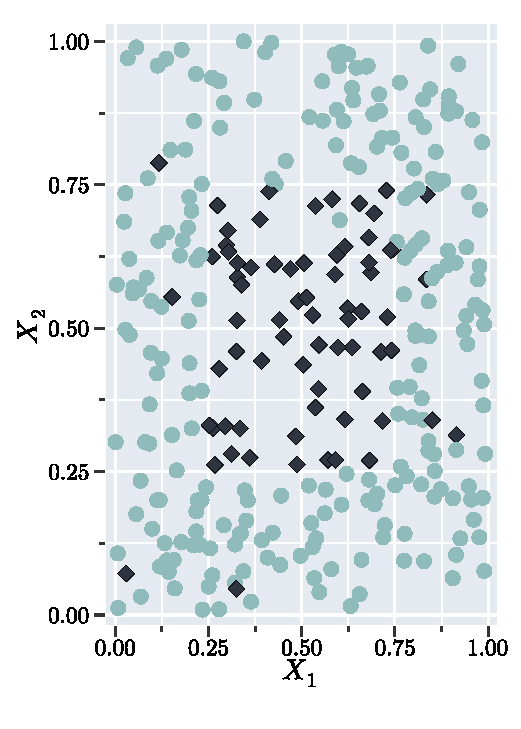
\includegraphics[width=\textwidth]{img/tree_obs.pdf} 
       \caption{Classification task on two features.}
       \label{fig:classification-task}
    \end{subfigure}
    \begin{subfigure}[t]{0.45\textwidth}
        \centering
        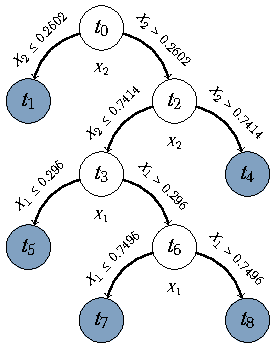
\includegraphics[width=\textwidth]{img/ctree.pdf}
        \caption{Resulting tree}
        \label{fig:tree-diagram}
    \end{subfigure}
    \caption{Classification task from the example represented}
    \label{figs:tree-example}
\end{figure}

Splitting rules will be crucial for developing the rest of this thesis, so we
must discuss them, even if only briefly. The true magic of the algorithm lies in
the splitting strategies and the termination criteria.

\subsection{Splitting rules}

\begin{dfn}{Split}{split}
    A \emph{split} $s$ of node $t$ is a partition of $\mathcal{X}_t$. Recall
    that the subset $\mathcal{X}_t$ is what we call a node. Formally, a
    partition is a collection of non-empty subsets of $\mathcal{X}_t$ such that:
    \begin{enumerate}
        \item The union of all subsets equals $\mathcal{X}_t$.
        \item The intersection of any two distinct subsets is empty.
    \end{enumerate}
\end{dfn}

The number of possible partitions of $\L_t$, with $N_t$ elements, into $k$
non-empty subsets is given by the Stirling number of the second kind
\cite{louppe2014}
\[
    S(N_t, k) \coloneqq \frac{1}{k!} \sum_{j=0}^{k} (-1)^{k-j} \binom{k}{j} j^{N_t}.
\]
Even in the case of binary partitions in which $S(N_t, k)$ reduces to $2^{N_t
-1}-1$, the number of partitions grows exponentially for the binary case. For
the non-binary case, even worse, it grows factorially. Calculating each possible
partition and choosing the best is computationally infeasible. The attentive
reader will find the similarities when describing in full detail the \ac{rl}
problem presented in Chapter \ref{chapter:ReinforcementLearning}. The best
binary split $s_*$ can be found using algorithm
\ref{alg:best-greedy-binary-split}.

\begin{algorithm}
    \SetKwFunction{GreedyBestSplit}{FindBestGreedyBinarySplit}
    \KwIn{A node $t$ (a subset $\L_t$ of the training set $\L$)}
    \KwOut{The best binary, greedy, split $s_*$ on $\L_t$}
    \Function{\GreedyBestSplit{$t$}}{
        $\Delta \gets - \infty$ \;
        \ForEach{feature $X_j$ with $j \in  \{1, \dots, p\}$}{
            Find the best greedy binary split $s_{*}^{j} \in \mathcal{Q}$ \label{line:best-greedy-split} \;
            \If{$\Delta i(s_{*}^{j}, t) > \Delta$}{
                $\Delta \gets \Delta i(s_{*}^{j}, t)$ \;
                $s_* \gets s_{*}^{j}$ \;
            }
        }
        \Return{$s_{*}$} \;
    }
    \caption[Best binary, greedy, split for node $t$.]{Best binary greedy split $s_*$ for node $t$ \cite[Ch.~3.6.3]{louppe2014}.}
    \label{alg:best-greedy-binary-split}
\end{algorithm}

In simple words, algorithm \ref{alg:best-greedy-binary-split} receives a node
$t$, which is nothing more than a subset of the training set. Then, it iterates
over the features of the data set, and finds the one that would yield a bigger
impurity decrease when split. In line \ref{line:best-greedy-split} of the
algorithm, the split $s_{*}^{j}$ is a question pertaining to the $j$-th feature.
If the $j$-th feature of the data set corresponded to the subject's age, one
suitable split would be ``is the subject older than 65?''. This question divides
the observations of the feature $X_j$ in two groups: those older and those
younger than 65. Once those two groups are established, we can calculate the
impurity decrease as the impurity of the current node, minus the weighted sum of
the impurities of the groups of individuals younger and older than 65.
Definition \ref{dfn:impurity-decrease} formalizes the process we just described.

It can be proved that the complexity of algorithm
\ref{alg:best-greedy-binary-split} is constrained by the complexity of the sort
operation used to order the values of $\Delta$ and retrieve the largest
\cite[Ch.~5]{louppe2014}.

With algorithm \ref{alg:best-greedy-binary-split}, we have enough background to
examine the similarities between the problem that arises from fitting a
classification tree and the more general reinforcement learning problem in part
\ref{part:II}.

\section{Bibliographical notes}
As mentioned, we had to skip several details necessary for an actual
implementation of the tree-fitting algorithm. They are not strictly mandatory
for the purposes of this thesis but are vastly interesting and worthwhile in
their own right. To clarify or expand upon the concepts presented here, please
refer to the sources used to develop this chapter:
\begin{enumerate}
    \item \citeauthor{breiman2017}'s book \citetitle{breiman2017}. One of the
        cornerstone texts for this subject and the first formal descriptions of
        the \ac{cart} algorithm \cite{breiman2017}.
    \item The standard textbook for modern machine learning algorithms and
        applications: \citetitle{elements2009}. This source is particularly good
        for reviewing the foundations of statistical, supervised learning in
        much more depth and in a better style that could be achieved here
        \cite{elements2009}.
    \item \citeauthor{louppe2014}'s doctoral thesis. Louppe is a core developer
        emeritus of the scikit-learn python library, the industry-standard
        library.  His work has valuable insights on the real-world
        considerations a practical implementation would have to keep in mind
        \cite{louppe2014}. After extensive research, this source provided the
        most satisfying treatment of classification and regression trees of all
        documents reviewed.
\end{enumerate}

The field of machine learning is so vast that we only had a chance to develop
the most rudimentary, essential ideas we will need. Reading the sources cited
for this chapter is encouraged.